\chapter{Implementation}
\label{ch:Implementation}
This chapter explains the detailed implementation of the methods described in \autoref{ch:Methodology}. It covers the specific processes, experiments, and analyses conducted. This includes the practical steps taken to prepare images, apply distortions, extract features, and train the models to assess image quality in teledermatology. \par

\section{Image Selection and Labeling Process}
\label{sec:ImgSelectLabel}
This section describes the initial stages of the implementation, focusing on the selection and preparation of the image datasets used in the study. \par

\subsection{Image Filtering and Selection}
\label{sub:ImgFilterSelect}
The first step in preparing the images involves carefully choosing good quality pictures from the SCIN and Fitzpatrick17k datasets. This selection is done manually to ensure that each image is clear and useful for clinical purposes. The primary focus during selection is on images that are well-framed and free of any distortions that might affect their usefulness in diagnosis. \par
\vspace{\baselineskip}
\noindent
Each selected image is checked to ensure it is not blurred, as clear images are crucial for accurate diagnosis. Additionally, it is important that the images have proper lighting and true contrast, meaning they should not be too bright or too dark. Proper lighting and contrast help in accurately showing the skin’s condition. Lastly, the images must represent realistic skin tones and colors because accurate color representation is critical for correct diagnoses. Some pictures from the dataset are included in the appendix for reference (see Appendix).\todo{maybe include some pictures in appendix} \par

\subsection{Labeling of the Test Set}
\label{sub:LabelingTestSet}
The labeling process involves manually scoring 200 images from the SCIN dataset. Of these 200, around 50 are good quality images, which I wanted to represent in the test set as well. Each image is scored on a scale from 0 to 1 for each criterion, where 0 indicates no distortion and 1 indicates extreme distortion. This manual labeling is done using a custom Python script \footnote{src/create\_labels.ipynb} \todo{correct this later}, which displays each image and prompts the user to enter scores for each distortion criterion. The scores are collected in a structured format and stored in a JSON file for later analysis. \par
\vspace{\baselineskip}
\noindent
This structured approach ensures consistent and thorough evaluation of each image. I did the labeling myself, using an absolute categorical rating method as described in \autoref{sub:SubjectiveQualityAssessment}. This method is very time consuming and requires significant effort from the evaluator. My labeling process involved scoring 200 images on 7 criteria each, resulting in 1400 labels. To ensure accuracy and avoid rushing, I deliberately spread out the labeling over multiple sessions.\par
\noindent
\subsubsection{Visualization of Label Distribution for the Test Set}
\label{subsub:LabelDist}
To understand the distribution of labels and how often distortions occur across different criteria, see \autoref{fig:DistTestCriteria}. These histograms are useful for visualizing the prevalence and severity of distortions in the dataset. The histograms are plotted with 10 bins for each criterion, where the first bin indicates no distortion, and the remaining bins represent increasing levels of distortion severity for that type. \par
\begin{figure}[ht]
    \centering
    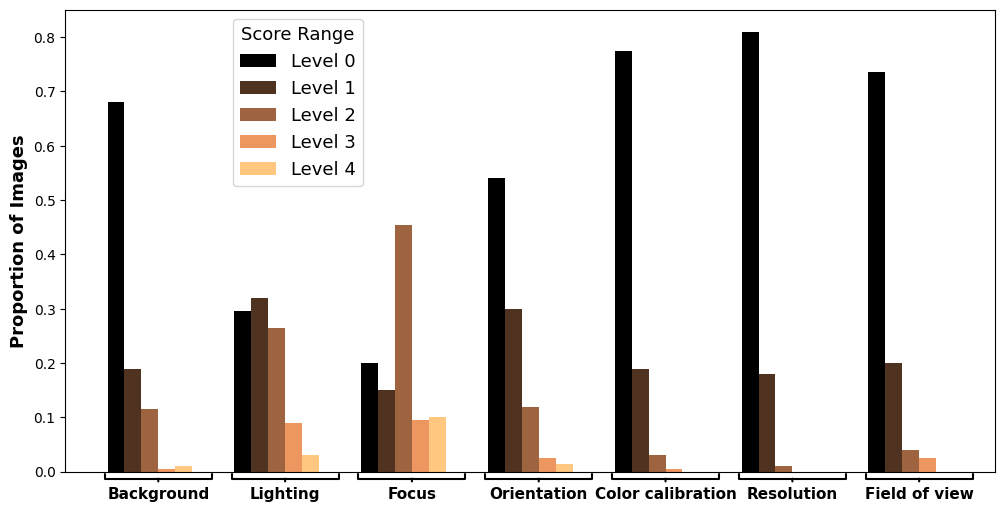
\includegraphics[keepaspectratio,width=15cm]{img/Distribution_test_criteria.png}
    \caption{Histograms showing the distribution of distortion scores for each quality criterion.}
    \label{fig:DistTestCriteria}
\end{figure}
\noindent
In \autoref{fig:DistTestCriteria} most criteria show a right-skewed distribution, indicating that higher levels of distortions are less common. This is evident in the criteria such as orientation, color calibration, background, resolution, and field of view. In contrast, the distributions for lighting and focus are more symmetrical, suggesting a more even spread of distortion severity levels. Since an image can have multiple distortions at once, it was difficult to separate them individually. For example, when an image is dark due to lighting issues, it becomes hard to judge other factors like focus, resolution, background, or color accuracy. These findings highlight the need to handle multiple distortions together during model training. They also point out the challenges in accurately labeling and assessing images that have several overlapping distortions. \par
\begin{figure}[ht]
    \centering
    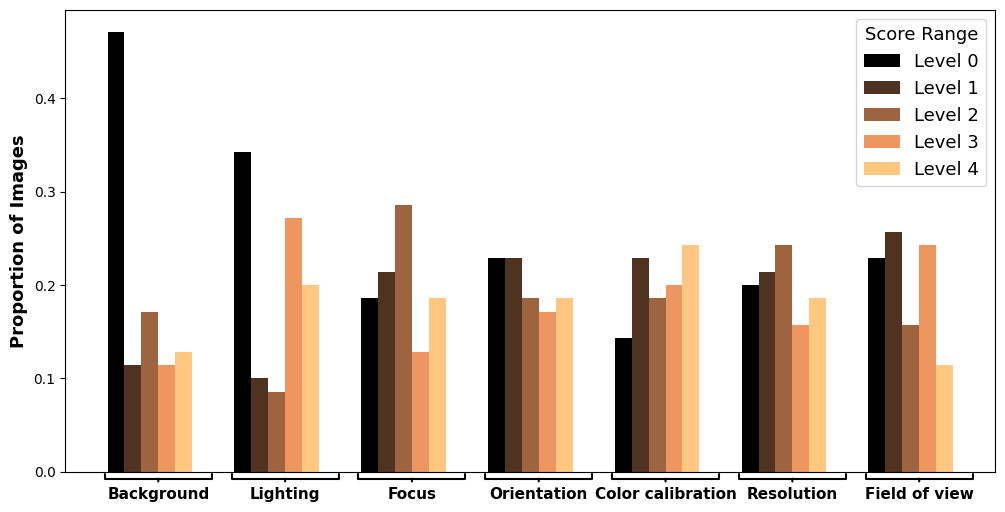
\includegraphics[keepaspectratio,width=15cm]{img/Distribution_test_criteria2.png}
    \caption{Histograms showing the distribution of distortion scores for each quality criterion.}
    \label{fig:DistTestCriteria2}
\end{figure}
\noindent
\section{Distortion Pipeline}
\label{sec:DistPipeline}
The distortion pipeline is central to simulating realistic image quality issues in teledermatology. Each quality criterion has multiple types of distortions, each having five levels of intensity, increasing in severity. All distortion types begin at zero, indicating no distortion applied, and progress to higher values that represent increasing levels of the specified distortion. Visual representations of the types of degradations at different ranges for each quality criterion are provided in \autoref{ch:Supplementary}.  \par

\subsection{Distortion Types}
\label{sub:DistTypes}
Here, each distortion type is briefly described, highlighting how they simulate different aspects of image degradation: \par
\begin{enumerate}
    \item Lighting:
        \begin{itemize}
            \item \textit{Brighten}: This operation increases the brightness of an image by applying color space transformations and adjustments, enhancing the overall visual intensity.
            \item \textit{Darken}: Similar to the brighten operation but reduces the visual intensity, making the image darker.
        \end{itemize}
    \item Focus:
        \begin{itemize}
            \item \textit{Gaussian blur}: Applies a Gaussian kernel to create a blurred effect, which softens the image by averaging the pixel values.
            \item \textit{Lens blur}: Uses a circular kernel to simulate the effect of a camera lens blur, causing a more uniform blur across the image.
            \item \textit{Motion blur}: Simulates the effect of motion, either from the camera or the subject, by applying a linear blur in a specified direction.
        \end{itemize}
    \item Orientation:
        \begin{itemize}
            \item \textit{Top perspective}: Alters the image to appear as if viewed from a higher angle, distorting the top part of the image.
            \item \textit{Bottom perspective}: Alters the image to appear as if viewed from a lower angle, distorting the bottom part of the image.
            \item \textit{Left perspective}: Alters the image to appear as if viewed from the left side, distorting the left part of the image.
            \item \textit{Right perspective}: Alters the image to appear as if viewed from the right side, distorting the right part of the image.
        \end{itemize}
    \item Color calibration:
        \begin{itemize}
            \item \textit{Color saturation 1}: Adjusts the saturation in the HSV color space, either increasing or decreasing the vividness of the colors.
            \item \textit{Color saturation 2}: Modifies the color channels in the LAB color space to change the saturation levels, affecting the color intensity.
        \end{itemize}
    \item Background:
        \begin{itemize}
            \item \textit{Color Block}: Uses skin segmentation to apply color block artifacts in the background, simulating background distortions and maintaining focus on the skin area.
        \end{itemize}
    \item Resolution:
        \begin{itemize}
            \item \textit{Change Resolution}: Alters the image resolution to simulate low-quality images by downsampling and then upsampling the image.
        \end{itemize}
    \item Field of view:
        \begin{itemize}
            \item \textit{Crop Image}: Crops the image to simulate different levels of field of view, reducing the visible area of the image.
        \end{itemize}
\end{enumerate}
\vspace{\baselineskip}
\noindent
The distortions for Lighting, Focus, and Color Calibration were adapted from the ARNIQA \autocite{ARNIQA} image degradation model, which was inspired by the KADID \autocite{KADID10k} dataset. These distortions originally provided an extensive range of severity levels. The severity levels were modified to better fit real-world distortions commonly encountered in teledermatology. The rest of the distortions were designed based on my own observations of real-world image quality issues in teledermatology. \par
\vspace{\baselineskip}
\noindent
For the orientation distortion, the perspective of the image is changed to simulate different viewing angles. By tilting, the image appears as if viewed from a higher, lower, left, or right angle. This gives the effect that the camera is not perpendicular to the skin, as if the camera was not held straight. For the resolution distortion was done by first downsampling the image to a lower resolution and then upsampling it back to its original size. This process simulates the effect of low-quality images by introducing pixelation and a loss of detail, similar to what happens when a low-resolution image is enlarged. For the field of view distortion, the image is cropped from the left corner to reduce the visible area. Normally, in good quality images, the skin lesion is centered. By cropping the corner, the lesion moves to the bottom right, simulating poor framing or incomplete capture of the lesion area. Lastly, the background distortion involved segmenting the skin from the background and depending on the amount of background present, color blocks are added to create a noisy background. This makes the background look noisy and cluttered, which can distract the model from focusing on the skin. This simulates real-world situations where the background is not clean, causing issues in image quality.\par

\section{Distortion Implementation Process}
\label{sec:DistProcess}

\begin{figure}[ht]
    \centering
    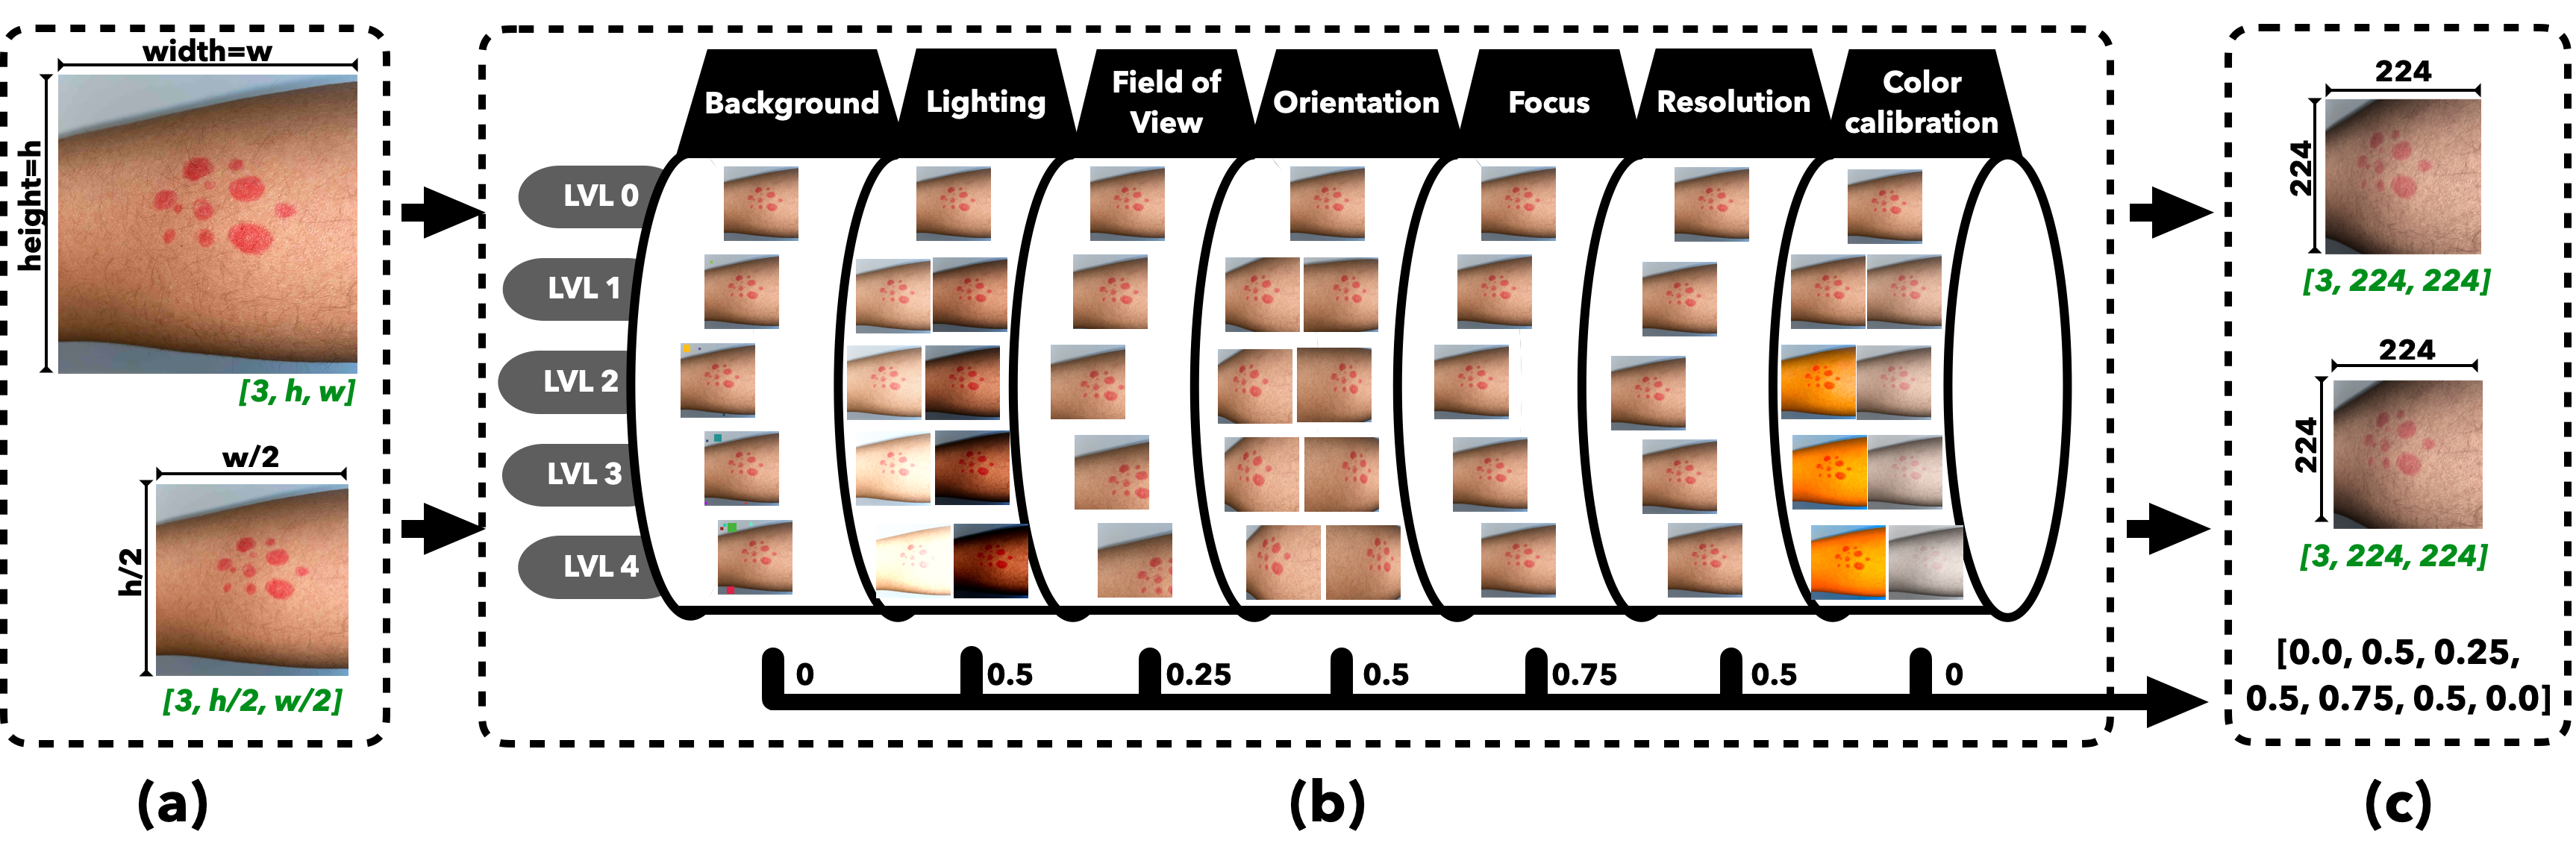
\includegraphics[keepaspectratio,width=15cm]{img/Distortion_pipeline.png}
    \caption{Distortion pipeline for generating training images with different levels of distortion. (a) shows the original image and its downscaled version. (b) illustrates the distortion pipeline where a type of distortion and a random level for each criterion are selected, with the corresponding mapped values shown at the bottom. (c) shows the output where the distorted original image and the distorted downscaled image are resized to 224x224 pixels, along with the 7 distortion values for the image.}
    \label{fig:DistPipeline}
\end{figure}

The distortion implementation process involves several key steps to create many realistic set of distorted images, which helps train and test the image quality assessment model. \par
\vspace{\baselineskip}
\noindent
For each image, the RGB version is taken and a downsampled version of the image at half the resolution is created. This involves resizing the image to half its original dimensions to simulate lower resolution. Distortions are then applied in a specific sequence (see \autoref{fig:DistPipeline}(b)) to ensure realistic simulation. The background distortion is applied first because it depends on identifying the skin area in the undistorted image. If the images have less than 10\% background in proportion to skin, no color blocks are added in the background. Therefore, the range value of 0 is used as value.  After that, other distortions are applied based on randomly chosen severity ranges. This ensures a variety of distortion levels across the dataset. \par
\vspace{\baselineskip}
\noindent
Once the distortions are applied, both the original and downsampled images are resized to 224x224 pixels to match the requirements for the backbone of ARNIQA \autocite{ARNIQA}. Following resizing, both images are normalized using the mean and standard deviation values of the ImageNet dataset (mean=[0.485, 0.456, 0.406], std=[0.229, 0.224, 0.225]). This normalization makes sure the images are processed consistently, as the model expects the images to have these properties, even though it might make the images look a bit different. \par
\vspace{\baselineskip}
\noindent
The severity of each applied distortion is mapped to a value between 0 and 1. This is done by taking the minimum and maximum possible values of the distortion and scaling the actual distortion value within this range. This standardized representation allows for consistent training and evaluation of the model later on. \par
\vspace{\baselineskip}
\noindent
This process can generate 3'750'000 possible combinations of distorted images because of the random selection of distortion types and severity levels. This highlights the robustness and adaptability of the pipeline. By following this detailed and structured approach, the distortion pipeline effectively simulates a wide range of real-world image quality issues in teledermatology, providing a comprehensive dataset for training and evaluating the image quality assessment model. \par

\section{Feature Extraction with the ARNIQA Backbone}
\label{sec:FeatureExtraction}
\begin{figure}[ht]
    \centering
    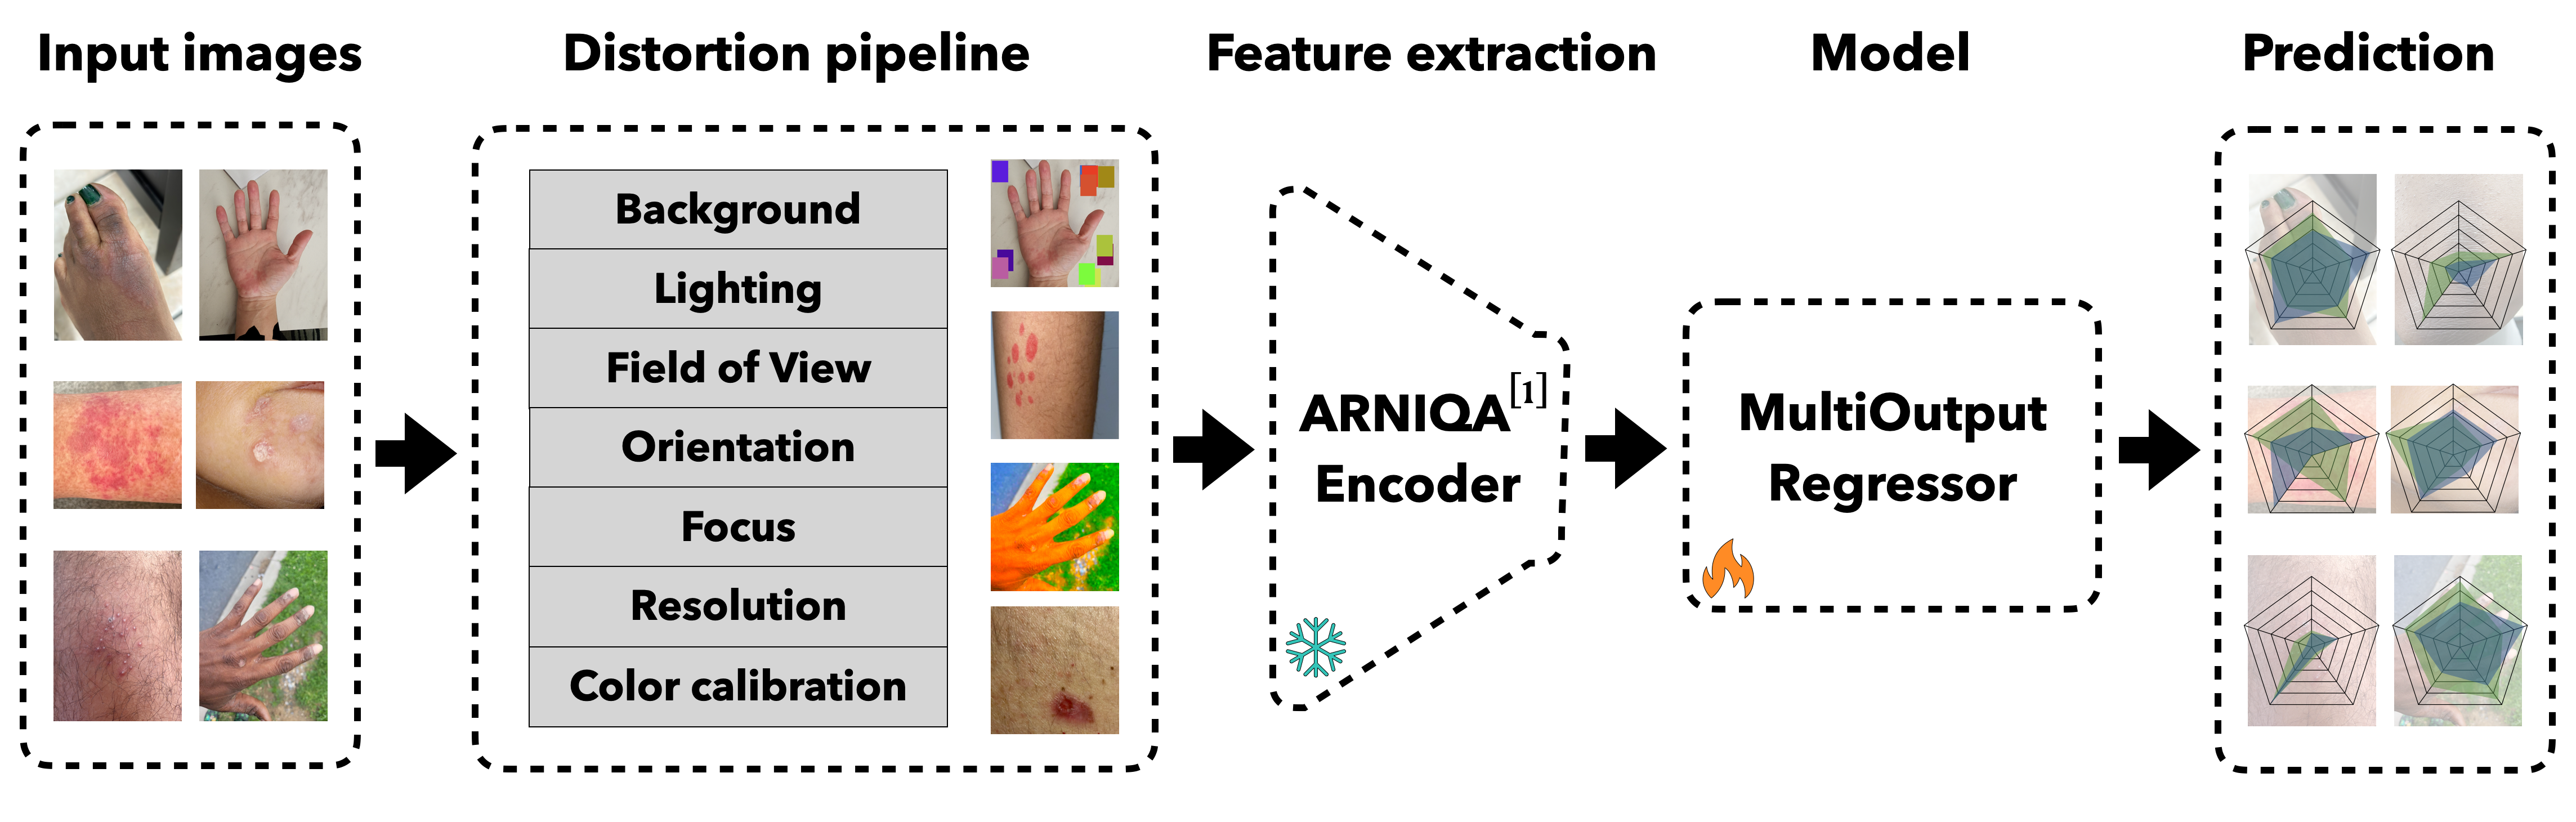
\includegraphics[keepaspectratio,width=15cm]{img/Architecture.png}
    \caption{Overview of the entire process for training and evaluating the image quality assessment model. (a) shows the album of input images. (b) depicts the distortion pipeline that randomly distorts images across seven criteria at five severity levels. (c) illustrates the feature extraction using the backbone from ARNIQA, which uses the SimCLR framework. (d) shows a scatter plot representing the model training process, with a diagonal red line indicating the fit. (e) presents the prediction results, comparing the model’s output to the actual labels.}
    \label{fig:Architecture}
\end{figure}

After creating the distortions and their half-scaled versions with mapped labels, the next step is to use the pretrained backbone from ARNIQA, which is loaded via \textit{torch.hub}. This pretrained model has already learned useful features from a large dataset, and these features are transferred to our specific task, a process known as transfer learning. This approach saves time and computational resources while improving the performance of the image quality assessment model. \par
\vspace{\baselineskip}
\noindent
The backbone from ARNIQA generates feature vectors that represent the distortion patterns in the images. By using both the original and downscaled images, the model effectively learns to distinguish between different levels of distortion. This dual-input method ensures a comprehensive understanding of image quality variations. \par
\vspace{\baselineskip}
\noindent
The extracted features, which have a shape of (\textit{num\_images}, 4096), and the target labels, representing distortion severity, which have a shape of (\textit{num\_images}, 7) corresponding to the seven distortion criteria, are then used to train the final image quality assessment model. \par

\section{Model Selection and Training}
\label{sec:ModelTraining}
Training was conducted using an NVIDIA A16 GPU with a maximum batch size of 10 for extracting features. This configuration, which includes 16GB vRAM, 1280 CUDA Cores, 40 3rd Gen Tensor Cores, and 512 GB RAM, ensured efficient utilization of GPU resources and expedited the training process. \par
\vspace{\baselineskip}
\noindent
To train the model, I started by creating multiple synthetically distorted images. The images were multiplied by factors of 4, 8, 16, 32, and 64 to examine how increasing the dataset size affected performance. It was hypothesized that larger datasets would lead to better performance. The dataset was then split into a training set (75\%) and a validation set (25\%) and experimented with three different multi-output models: XGBRegressor, an XGBClassifier, and both MLP Regressor and MLP Classifier. These models were chosen because they handle complex relationships well and can predict multiple outputs at once.\par
\vspace{\baselineskip}
\noindent
The XGBRegressor and XGBClassifier were selected for their ability to handle large datasets and find complex patterns effectively. The regressor predicts continuous scores for each quality criterion, while the classifier categorizes these scores into predefined levels. The MLP Regressor and Classifier, which are neural networks, were chosen for their ability to learn detailed patterns through multiple layers. \par
\vspace{\baselineskip}
\noindent
To optimize the hyperparameters of the models, I used the Weights and Biases\footnote{\url{https://wandb.ai/site}} tool to perform a hyperparameter sweep. This involved randomly searching for the best hyperparameters, aiming to maximize the overall Spearman’s Rank Order Correlation Coefficient (SRCC). The hyperparameters were saved in \textit{.npy} files for features and scores to ensure reproducibility and to avoid repeatedly going through the distortion pipeline and feature extraction when training different models. \par
\vspace{\baselineskip}
\noindent
Each model was trained using different multiples of the dataset, such as 4, 8, 16, 32, and 64, to examine how increasing the dataset size affected performance. It was hypothesized that larger datasets would improve model performance, although this hypothesis is to be confirmed through plotting and analysis. \par
\vspace{\baselineskip}
\noindent
The following parameters were considered for XGB and MLP models: \par
\vspace{\baselineskip}
\noindent
XGB Parameters:
\begin{itemize} 
    \item \textit{n\_estimators}: Number of trees in the ensemble.
    \item \textit{max\_depth}: Maximum depth of each tree.
    \item \textit{learning\_rate}: Step size shrinkage used to prevent overfitting.
    \item \textit{subsample}: Fraction of samples used for fitting the individual trees.
    \item \textit{early\_stopping\_rounds}: Rounds of early stopping.
    \item \textit{gamma}: Minimum loss reduction required to make a further partition.
    \item \textit{min\_child\_weight}: Minimum sum of instance weight needed in a child.
    \item \textit{reg\_alpha}: L1 regularization term on weights (fixed value of 0).
    \item \textit{reg\_lambda}: L2 regularization term on weights (fixed value of 1).
    \item \textit{tree\_method}: Algorithm used for learning and training (fixed value 'hist').
    \item \textit{objective}: Objective function to minimize (specific to XGBRegressor).
    \item \textit{n\_jobs}: Number of parallel threads used to run XGBoost (specific to XGBRegressor).
    \item \textit{multi\_strategy}: Strategy for handling multiple outputs (specific to XGBRegressor).
    \item \textit{booster}: Type of boosting model to use (specific to XGBClassifier).
    \item \textit{eval\_metric}: Evaluation metric(s) to be used for validation (specific to XGBClassifier).
\end{itemize}
\noindent
MLP Parameters:
\begin{itemize}
    \item \textit{hidden\_layer\_sizes}: The number of neurons in the hidden layers.
    \item \textit{activation}: Activation function for the hidden layer (fixed value 'relu').
    \item \textit{alpha}: L2 regularization term.
    \item \textit{solver}: Optimization algorithm for weight optimization (fixed value 'adam').
    \item \textit{learning\_rate\_init}: Initial learning rate.
    \item \textit{max\_iter}: Maximum number of iterations.
    \item \textit{early\_stopping}: Whether to use early stopping to terminate training when validation score is not improving (fixed value True).
\end{itemize}
\vspace{\baselineskip}
\noindent
To improve the generalization of the model and prevent it from memorizing the training data, I used L2 regularization and subsampling. L2 regularization helps to avoid large coefficients, and subsampling trains the model on different subsets of data to reduce variance. \par
\vspace{\baselineskip}
\noindent
The models were trained individually on the SCIN and Fitzpatrick datasets and on a combination of both datasets to assess performance. The best model, which provided good scores across all seven distortion criteria, was selected for further testing. Predictions from the regressor were clipped to the range of 0 to 1 to ensure they were within valid bounds. The scores were then binarized using a function that converts continuous scores to categorical ones based on defined thresholds. This helps in categorizing the severity levels effectively.\par

\subsection{Hyperparameter Configuration}
\label{sub:HyperparamConfig}
The following table shows the configurations used in the hyperparameter sweep: \par
\begin{table}[h]
    \centering
    \begin{tabular}{|l|l|}
        \hline
        \textbf{XGB Parameter} & \textbf{Values} \\
        \hline
        \textit{model\_type} & [xgb\_reg, xgb\_cls] \\
        \textit{batch\_size} & 10 \\
        \textit{num\_distortions} & [4, 16, 64] \\
        \textit{n\_estimators} & [50, 100, 200, 300] \\
        \textit{learning\_rate} & \{"min": 0.0001, "max": 0.1\} \\
        \textit{min\_child\_weight} & \{"min": 1, "max": 150\} \\
        \textit{early\_stopping\_rounds} & [10, 20, 30, 40] \\
        \textit{subsample} & [0.5, 0.6, 0.7, 0.8, 0.9, 1.0] \\
        \textit{max\_depth} & [3, 5, 7, 9] \\
        \textit{gamma} & \{"min": 0.001, "max": 0.5\} \\
        \textit{multi\_strategy} & [one\_output\_per\_tree, multi\_output\_tree] \\
        \hline
    \end{tabular}
    \caption{Hyperparameter Configurations for XGB Models}
    \label{table:xgb_hyperparams}
\end{table}

\begin{table}[h]
    \centering
    \begin{tabular}{|l|l|}
        \hline
        \textbf{MLP Parameter} & \textbf{Values} \\
        \hline
        \textit{model\_type} & [mlp\_reg, mlp\_cls] \\
        \textit{batch\_size} & 10 \\
        \textit{num\_distortions} & [4, 16, 64] \\
        \textit{hidden\_layer\_sizes} & [(512,), (1024,), (512, 256), (1024, 512), (512, 512)] \\
        \textit{activation} & relu \\
        \textit{alpha} & \{"min": 0.0001, "max": 0.01\} \\
        \textit{learning\_rate\_init} & \{"min": 0.0001, "max": 0.1\} \\
        \textit{max\_iter} & [200, 300, 500] \\
        \hline
    \end{tabular}
    \caption{Hyperparameter Configurations for MLP Models}
    \label{table:mlp_hyperparams}
\end{table}
\vspace{\baselineskip}
\noindent
By following this comprehensive approach, the models were thoroughly evaluated and optimized, ensuring robust performance in assessing the quality of teledermatology images. \par

\subsection{Performance Metrics and Visualization}
\label{sub:PerfMetrics}
To thoroughly understand how well the model performs, both overall metrics and individual criteria performance were analyzed\footnote{from utils.visualization import print\_metrics}. This approach helps in identifying which specific quality criteria the model handles well and which ones it struggles with. \par
\vspace{\baselineskip}
\noindent
In addition to looking at the numerical metrics, visual tools were used for a clearer picture. For each criterion, a confusion matrix\footnote{from utils.visualization import plot\_all\_confusion\_matrices} was created. This matrix shows where the model makes correct predictions and where it makes mistakes, giving a detailed view of its accuracy for each type of distortion. Another important visualization was the plot of predicted versus actual values\footnote{from utils.visualization import plot\_prediction\_scores}. In this plot, the actual values are on the x-axis and the predicted values are on the y-axis. A diagonal line represents perfect predictions, showing where the predicted values match the actual values exactly. Additionally, a mean line of the predictions and a shaded area indicating the standard deviation were included. This plot helps in seeing how close the predictions are to the actual values and how much variability there is in the predictions. \par

\section{Model Testing}
\label{sec:ModelTesting}
After training the models on the SCIN and Fitzpatrick datasets, and on a combination of both, I tested their generalizability. This involved seeing how well the models trained on SCIN performed on the Fitzpatrick dataset and vice versa. I also evaluated the models using a combined dataset to find the best one that performed well across all seven types of distortions. \par
\vspace{\baselineskip}
\noindent
The best model was then tested on two specific sets of images. The first set included 70 images that were distorted using a pipeline to create consistent types of distortions. This was to see how well the model handled these controlled distortions. The second set included 200 images that had authentic distortions. This allowed me to compare the model’s performance with my own evaluations. \par
\vspace{\baselineskip}
\noindent
The test images went through similar preprocessing steps as during training: half-scaling the image, resizing it to 224x224, and normalizing it. They were then passed through the backbone of ARNIQA to extract features before being tested on the final model. The only step not performed was distorting the images. Instead, the scores for the 200 images were loaded from a JSON\footnote{src/test\_200/scores.json} file, and the scores for the 70 images were loaded from a \textit{scores.npy}\footnote{src/test\_70/embeddings/scores.npy} file. \par
\vspace{\baselineskip}
\noindent
To validate my approach, I also tested both sets of images using ARNIQA, a known quality assessment model. ARNIQA provided a quality score between 0 and 1, with higher scores indicating better image quality. This comparison helped determine if the synthetic distortions improved the model’s performance. \par
\subsection{Visualizing the Tests}
\label{sub:VizModelPerformance}
To understand the model’s performance better, I created visualizations\footnote{from utils.visualization import plot\_results}. For the 70 images from the distortion pipeline, I used a four-column layout. The first column showed the original image, the second showed the distorted image, the third showed the actual labels, and the fourth showed the model’s predictions. This setup made it easy to see how well the model’s predictions matched the actual distortions. \par
\vspace{\baselineskip}
\noindent
For the 200 images with authentic distortions, I used a three-column layout. The first column showed the image, the second column displayed my labels, and the third column showed the model’s predictions. This comparison helped me see how well the model’s predictions aligned with my evaluations. \par
\vspace{\baselineskip}
\noindent
These visualizations provided a clear picture of the model’s performance, showing its strengths and areas where it could improve. \par